
\documentclass[10pt,a4paper]{jsarticle}
\usepackage{robomech}
\usepackage[dvips]{graphicx}
\usepackage{tabularx,amsmath,amssymb}
\usepackage{txfonts,bm}
%\usepackage{flushend}
%
\title{人語を話す知的ハムスター「はむこ」の \\
類似経験を持つハムスターとの対話を通じた当事者研究}
\engtitle{Talking Intellectual Hamster "Hamko": \\ 
Studying oneself through communication with other hamsters who share similar experiences 
}
\author{
○学\hspace{1zw}若田部 亮 (東京大学)\hspace{2zw}
公\hspace{1zw}いんてる はむこ (東京大学)}

\engauthor{%
*Ryo WAKATABE, The University of Tokyo, wakataberyo@gmail.com \\
 Hamko INTEL, The University of Tokyo, @ryo\_wk }
% 英語のabst
\abstract{
Hamsters are not thought to speak.
%
Recently, we, hamsters, realize we can speak, especially in Japanese. 
%
However, no research indicates hamsters can speak.
%
Here, I investigate our speaking skill by talking each other.
%
We recorded all 3-days convesations by audio microphones.
%
As a result, we found that the ability to speak in Japanese is 20\% higher than avaratge Japanese people.
%
Moreover, we suggest that we, hamsters, should take all over the world.
}
% キーワード
\keyword{Hamster, Speaking, Linguistic Ability, World Conquiring }
%


\begin{document}
\setlength{\baselineskip}{4.685truemm}% 52 line
\maketitle
\thispagestyle{empty}

% Intro Section
\section{研究背景と目的}

目的 \cite{Cornwell1975175, 110002427721}


% Method Section
\section{方法}
\subsection{被験者}
\subsection{計測方法}

\section{計測実験}
\subsection{目的と方法}

\begin{itemize}
    \item[A.] アイテム1
    \item[B.] アイテム2
    \item[C.] アイテム3
\end{itemize}

\subsection{結果}
意味のない結果は、何ら意味を持たない(\figref{fig:meaningless}).

\begin{figure}[t!]
 \centering
  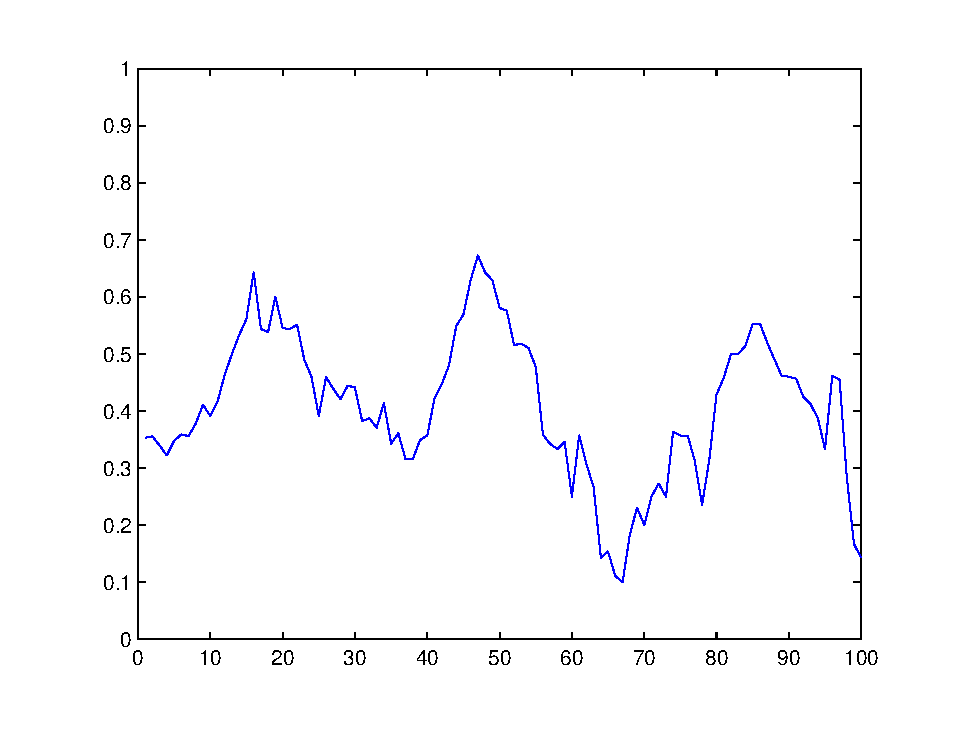
\includegraphics[width=0.40\textwidth]{figure/sample.eps}
 \caption{Meaningless figure.}
 \label{fig:meaningless}
\end{figure}


\section{結論}


%以下引用
\begin{footnotesize}
\bibliographystyle{IEEEtranS}
%\bibliographystyle{junsrt}
\bibliography{/home/hamko/git/bibtex/thesis}
\end{footnotesize}

\end{document}
